\documentclass[11pt]{article}
\usepackage{calc}
\usepackage[margin={1in,0.5in},footskip=0in]{geometry}
\usepackage[miniquiz]{hwk}
\usepackage{tikz, pgfplots}

\renewcommand{\theclass}{math 1300}
\renewcommand{\dateinfo}{December 11, 2012}
\renewcommand{\theassignment}{Quiz 11}

\pgfplotsset{compat=1.7}

\begin{document}
\pagestyle{empty}
\newsavebox{\quizfront}
\begin{lrbox}{\quizfront}
\begin{minipage}[top][4.5in][t]{\textwidth} \setlength{\parindent}{1.5em}
\drawtitle
\vspace{-0.5in}
\begin{enumerate}

\item Suppose $f(x)$ is odd. What is the average value of $f(x)$ from
  $-2$ to 2?
  \vfill
  {\color{blue}
    
    Since $f(x)$ is odd we know that $\int_{-2}^2 f(x)\; dx = 0$, so
    \[
    \text{Average Value} = \frac{1}{2-(-2)}\int_{-2}^2 f(x)\; dx = 0.
    \]

  }
  \vfill


\end{enumerate}

%\vfill

%\hfill\textsc{over} $\longrightarrow$


\end{minipage}
\end{lrbox}

%%%%%%%%%%%%%%%%%%%%%%%%%%%%%%%%%%%%%%%%%%%%%%%%%%%%%%
%%%% This is for the back of the quiz
%%%%%%%%%%%%%%%%%%%%%%%%%%%%%%%%%%%%%%%%%%%%%%%%%%%%%%
\newsavebox{\quizback}
\begin{lrbox}{\quizback}
\begin{minipage}[top][4.5in][t]{\textwidth} \setlength{\parindent}{1.5em}
\begin{enumerate}

\item[2.] The graph of $f(x)$ is shown below. If $F'(x)=f(x)$ and
  $F(0) = 3$, find the coordinates of an inflection point of $F$.

  \begin{center}
    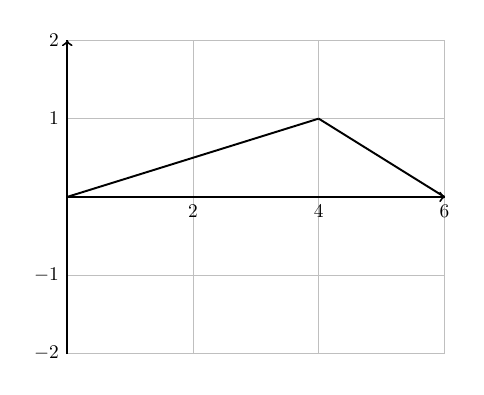
\begin{tikzpicture}[scale=0.7]
      \begin{axis}[  
	axis x line=middle, axis y line=middle,
	axis line style={->}, 
	tick style={color=black},
	xmin=0,
	xmax=6.01,
	ymin=-2.01,
	ymax=2,
	xtick={0,2,4,6},
	ytick={-2,-1,0,1,2},
	major tick length={1},
	grid=major,
	line width=1pt,] 
	\plot[smooth, domain=0:4] {x/4}; 
	\plot[smooth, domain=4:6] {3-x/2}; 
      \end{axis}
    \end{tikzpicture}
  \end{center}

  \vfill
  {\color{blue}
    
    An inflection point of $F(x)$ is where $F(x)$ changes concavity.
    This occurs when $F'(x) = f(x)$ changes from increasing to
    decreasing or from decreasing to increasing.  We see that this
    happens at $x = 4$.  Then
    \begin{align*}
      F(4) - F(0) &= \int_0^4 f(x)\; dx \\
      F(4) - 3 &= 2\\
      F(4) &= 5,
    \end{align*}
    so $F(x)$ has an inflection point at $(4,5)$.

  }
  \vfill

  
\end{enumerate}
\end{minipage}
\end{lrbox}

%%%%%%%%%%%%%%%%%%%%%%%%%%%%%%%%%%%%%%%%%%%%%%%%%%%%%%
%%%%
%%%% Now we make two copies of the ``quizfront'' box
%%%%
%%%%%%%%%%%%%%%%%%%%%%%%%%%%%%%%%%%%%%%%%%%%%%%%%%%%%%%
\noindent \usebox{\quizfront}

\noindent \usebox{\quizback}

%%%% Uncomment the rest to have a two-sided quiz.
%\pagebreak
%\noindent \usebox{\quizback}
%\vfill
%\noindent \usebox{\quizback}
\end{document}